\documentclass{article}
\usepackage{tikz}
\usepackage{multicol}
\usepackage[margin=1in]{geometry}

\begin{document}

\pagestyle{empty}
\centerline{\Large \sffamily Math 125: Epidemiology}

\bigskip

\centerline{\Large \sffamily \bfseries In-Class Activity: Standardization \& Age Adjustment}

\vspace*{.25in}
The graph shows some imaginary mortality statistics for several countries.  For the sake of simplicity, the age-dependence of mortality is reduced to just two groups: young people age 40 and below, and older people age 41 and above.  


\bigskip

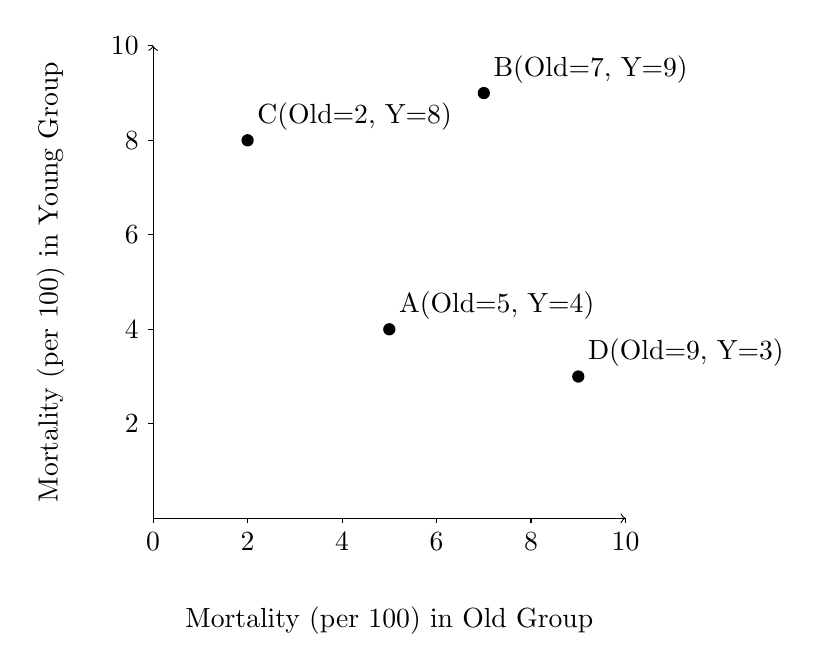
\begin{tikzpicture}[scale=.6]
\draw[->,black] (0,0) -- (10,0) node[pos=.5,below=1cm] {Mortality (per 100) in Old Group};
    % Put some ticks and tick labels in:
    \foreach \x in {0,2,4,6,8,10}
    \draw (\x,0) -- (\x,-0.1) node[below] {$\x$};

\draw[->,black] (0,0) -- (0,10) node[pos=.5,above=1cm,sloped] {Mortality (per 100) in Young Group};
    % Put some ticks and tick labels in:
    \foreach \y in {2,4,6,8,10}
    \draw (0,\y) -- (-.1,\y) node[left] {$\y$};

\foreach \x/\y/\t in {5/4/A,7/9/B,2/8/C,9/3/D}
{
  \fill (\x,\y) circle(1.3mm) ;

\node at (\x,\y) [anchor=south west] {\t (Old=\x, Y=\y)};
};
\end{tikzpicture}

\begin{multicols}{2}

\begin{enumerate}
\item Calculate the overall mortality {\bf rate} (per 1000) in each country.  Assume that the populations are as 
follows:

\centerline{\begin{tabular}{c|rr}
Country & Old & Young \\\hline
A & 200 & 800 \\
B & 100 & 900 \\
C & 600 & 400 \\
D & 400 & 100 \\
\multicolumn{3}{c}{Population}\\
\end{tabular}}

Write down the countries in order from best to worst.

\bigskip

\item Calculate an age-adjusted mortality rate for each country.  Take this as the standard population

\centerline{\begin{tabular}{c|rr}
Country & Old & Young \\\hline
Standard Pop. & 400 & 600 \\
\end{tabular}}

Write down the countries in order from best to worst.

\columnbreak

\item Calculate years of potential life lost in each country.
For the sake of the calculation, assume that the typical age of the young people is 20 years, versus 60 years for the older people.  Use 65 years as the reference age.

Write down the countries in order from best to worst.

\bigskip

\end{enumerate}

\end{multicols}

\end{document}